\documentclass[12pt,a4paper]{article}
\usepackage[UTF8]{ctex}
\usepackage{amsmath}
\usepackage{amssymb}
\usepackage{graphicx}
\usepackage{booktabs}
\usepackage{multirow}
\usepackage{listings}
\usepackage{xcolor}
\usepackage{geometry}
\usepackage{float}
\usepackage{subfigure}
\usepackage{hyperref}
\usepackage{textcomp}
\usepackage{pmboxdraw}
\usepackage{tikz}
\usetikzlibrary{arrows.meta, shapes.geometric, shapes.misc}

% 添加以下包来支持Unicode字符
\usepackage{fontspec}
\usepackage{unicode-math}

% 支持希腊字符的字体
\newfontfamily\greekcodefont{DejaVu Sans Mono}[
    Scale=0.9
]

\newcommand{\gepsiv}{{\greekcodefont\textcolor{green!60!black}{ε}}}
\newcommand{\gsigmax}{{\greekcodefont\textcolor{green!60!black}{σ}}}
\newcommand{\gsigmay}{{\greekcodefont\textcolor{green!60!black}{σ}}}
\newcommand{\gtauxy}{{\greekcodefont\textcolor{green!60!black}{τ}}}
\newcommand{\gnu}{{\greekcodefont\textcolor{green!60!black}{ν}}}
\newcommand{\galpha}{{\greekcodefont\textcolor{green!60!black}{α}}}
\newcommand{\gbeta}{{\greekcodefont\textcolor{green!60!black}{β}}}
\newcommand{\ggamma}{{\greekcodefont\textcolor{green!60!black}{γ}}}
\newcommand{\gdelta}{{\greekcodefont\textcolor{green!60!black}{δ}}}

\geometry{left=2.5cm,right=2.5cm,top=2.5cm,bottom=2.5cm}

% 代码样式设置
\lstset{
    language=C++,
    basicstyle=\ttfamily\small,          % 保持原有字体
    keywordstyle=\color{blue},
    commentstyle=\color{green!60!black},  % 保持原有注释样式
    stringstyle=\color{red},
    numbers=left,
    numberstyle=\tiny\color{gray},
    frame=single,
    breaklines=true,
    captionpos=b,
    escapeinside={(*@}{@*)},             % 添加这一行:允许在代码中嵌入LaTeX命令
    columns=flexible,
    keepspaces=true,
    showstringspaces=false
}

\title{\textbf{STAPpp程序T3三角形单元扩展实验报告}}
\author{清华大学行健书院 \\ 有限元法基础课程大作业 \\ 
        \textbf{姓名:}吴致远 \quad \textbf{学号:}2022013266 \quad \textbf{班级:}行健-力2}
\date{\today}

\begin{document}

\maketitle

\tableofcontents
\newpage

\section{实验概述}

\subsection{实验目的}

本实验旨在扩展STAPpp有限元程序功能,新增T3三角形单元类型,通过理论推导、程序实现和数值验证的完整过程,达到以下目标:

\begin{enumerate}
    \item 深入理解T3三角形单元的理论基础和数学推导过程
    \item 基于面向对象编程思想,在STAPpp框架下实现完整的T3单元类
    \item 设计并实施包括分片试验、收敛性分析和工程验证在内的完整验证体系
    \item 通过数值实验验证T3单元实现的正确性和可靠性
    \item 掌握有限元程序设计的基本方法、调试技巧和验证策略
\end{enumerate}

\subsection{实验意义与应用价值}

T3三角形单元作为平面有限元分析中最基础的单元类型之一,具有重要的理论价值和工程应用意义:

\begin{itemize}
    \item \textbf{几何适应性强}:能够处理任意复杂的几何边界,适用于不规则区域的离散化
    \item \textbf{理论基础完备}:应变为常数,便于理论分析和数学推导
    \item \textbf{编程实现简单}:单元刚度矩阵可解析求解,无需数值积分
    \item \textbf{工程应用广泛}:在商业软件如ANSYS、ABAQUS中得到广泛应用
    \item \textbf{扩展性良好}:为高阶单元和多物理场耦合分析奠定基础
\end{itemize}

通过T3单元的完整实现过程,可以深入理解有限元法的核心概念、程序设计方法和数值验证策略,为后续研究和工程应用打下坚实基础。

\section{理论基础}

\subsection{T3单元几何描述与坐标系统}

T3单元是具有3个节点的三角形单元,每个节点具有2个平移自由度($u_x$ 和 $u_y$)。单元在全局坐标系 $(x,y)$ 中的几何形状由3个节点坐标 $(x_i, y_i)$($i=1,2,3$)唯一确定。

% filepath: /home/wiz/WorkSpace/STAPpp/writing/main.tex
\begin{figure}[H]
\centering
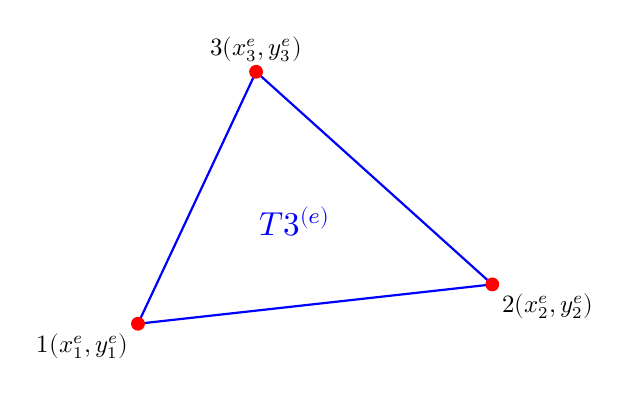
\begin{tikzpicture}[scale=1.0]
    % 定义三个节点(不规则三角形)
    \coordinate (A) at (0,0);
    \coordinate (B) at (4.5,0.5);
    \coordinate (C) at (1.5,3.2);
    
    % 绘制三角形
    \draw[thick, blue] (A) -- (B) -- (C) -- cycle;
    
    % 标记节点(红色圆点)
    \fill[red] (A) circle (2.5pt);
    \fill[red] (B) circle (2.5pt);
    \fill[red] (C) circle (2.5pt);
    
    % 节点编号和坐标标注
    \node[below left, font=\small] at (A) {$1(x_1^e, y_1^e)$};
    \node[below right, font=\small] at (B) {$2(x_2^e, y_2^e)$};
    \node[above, font=\small] at (C) {$3(x_3^e, y_3^e)$};
    
    % 在顶点处标注节点编号
    % \node[white, font=\footnotesize\bfseries] at (A) {1};
    % \node[white, font=\footnotesize\bfseries] at (B) {2};
    % \node[white, font=\footnotesize\bfseries] at (C) {3};
    
    % 单元标识
    \node[blue, font=\large] at (2,1.3) {$T3^{(e)}$};
    
    % % 添加坐标轴(可选)
    % \draw[->, gray] (-0.5,0) -- (5.5,0) node[right, black] {$x$};
    % \draw[->, gray] (0,-0.5) -- (0,4) node[above, black] {$y$};
    % \node[below left, gray] at (0,0) {$O$};
\end{tikzpicture}
\caption{T3三角形单元节点编号与坐标系统}
\label{fig:t3_geometry}
\end{figure}

\subsection{形函数推导与面积坐标}

T3单元的形函数基于面积坐标理论,具有明确的几何意义。形函数的数学表达为:

\begin{equation}
N_i = \frac{1}{2A}(a_i + b_i x + c_i y), \quad i=1,2,3
\end{equation}

其中,$A$为三角形面积,通过行列式计算:

\begin{equation}
A = \frac{1}{2}\begin{vmatrix}
1 & x_1 & y_1 \\
1 & x_2 & y_2 \\
1 & x_3 & y_3
\end{vmatrix}
\end{equation}

形函数系数$a_i$、$b_i$、$c_i$的计算公式为:

\begin{align}
a_1 &= x_2y_3 - x_3y_2, \quad b_1 = y_2 - y_3, \quad c_1 = x_3 - x_2 \\
a_2 &= x_3y_1 - x_1y_3, \quad b_2 = y_3 - y_1, \quad c_2 = x_1 - x_3 \\
a_3 &= x_1y_2 - x_2y_1, \quad b_3 = y_1 - y_2, \quad c_3 = x_2 - x_1
\end{align}

形函数具有重要的数学性质:
\begin{itemize}
    \item \textbf{配分性质}:$\sum_{i=1}^3 N_i = 1$
    \item \textbf{插值性质}:$N_i(x_j, y_j) = \delta_{ij}$
    \item \textbf{线性完备性}:能够精确表示线性位移场
\end{itemize}

\subsection{应变-位移关系与应变矩阵}

单元内任意点的位移场通过形函数插值表示:

\begin{equation}
\begin{bmatrix} u_x \\ u_y \end{bmatrix} = \sum_{i=1}^{3} N_i \begin{bmatrix} u_{xi} \\ u_{yi} \end{bmatrix}
\end{equation}

基于小变形假设,应变分量定义为:

\begin{equation}
\varepsilon_x = \frac{\partial u_x}{\partial x}, \quad \varepsilon_y = \frac{\partial u_y}{\partial y}, \quad \gamma_{xy} = \frac{\partial u_x}{\partial y} + \frac{\partial u_y}{\partial x}
\end{equation}

应变矩阵$\mathbf{B}$为:

\begin{equation}
\mathbf{B} = \frac{1}{2A} \begin{bmatrix}
b_1 & 0 & b_2 & 0 & b_3 & 0 \\
0 & c_1 & 0 & c_2 & 0 & c_3 \\
c_1 & b_1 & c_2 & b_2 & c_3 & b_3
\end{bmatrix}
\end{equation}

\subsection{本构关系与弹性矩阵}

对于平面应力问题,应力-应变关系由广义胡克定律描述:

\begin{equation}
\begin{bmatrix} \sigma_x \\ \sigma_y \\ \tau_{xy} \end{bmatrix} = \mathbf{D} \begin{bmatrix} \varepsilon_x \\ \varepsilon_y \\ \gamma_{xy} \end{bmatrix}
\end{equation}

弹性矩阵$\mathbf{D}$为:

\begin{equation}
\mathbf{D} = \frac{E}{1-\nu^2} \begin{bmatrix}
1 & \nu & 0 \\
\nu & 1 & 0 \\
0 & 0 & \frac{1-\nu}{2}
\end{bmatrix}
\end{equation}

\subsection{单元刚度矩阵推导}

根据虚功原理,单元刚度矩阵通过以下积分计算:

\begin{equation}
\mathbf{K}^e = \int_{\Omega^e} \mathbf{B}^T \mathbf{D} \mathbf{B} \,d\Omega
\end{equation}

由于T3单元的应变矩阵$\mathbf{B}$在单元内为常数,积分可以解析计算:

\begin{equation}
\mathbf{K}^e = t \cdot A \cdot \mathbf{B}^T \mathbf{D} \mathbf{B}
\end{equation}

其中$t$为单元厚度,$A$为单元面积。

\section{程序设计与实现}

\subsection{STAPpp程序架构分析}

STAPpp采用面向对象的C++设计模式,具有良好的模块化结构和扩展性。主要类层次结构如图\ref{fig:stap_architecture}所示。

% filepath: /home/wiz/WorkSpace/STAPpp/writing/main.tex
% 将第218行开始的TikZ图形替换为以下内容:

\begin{figure}[H]
\centering
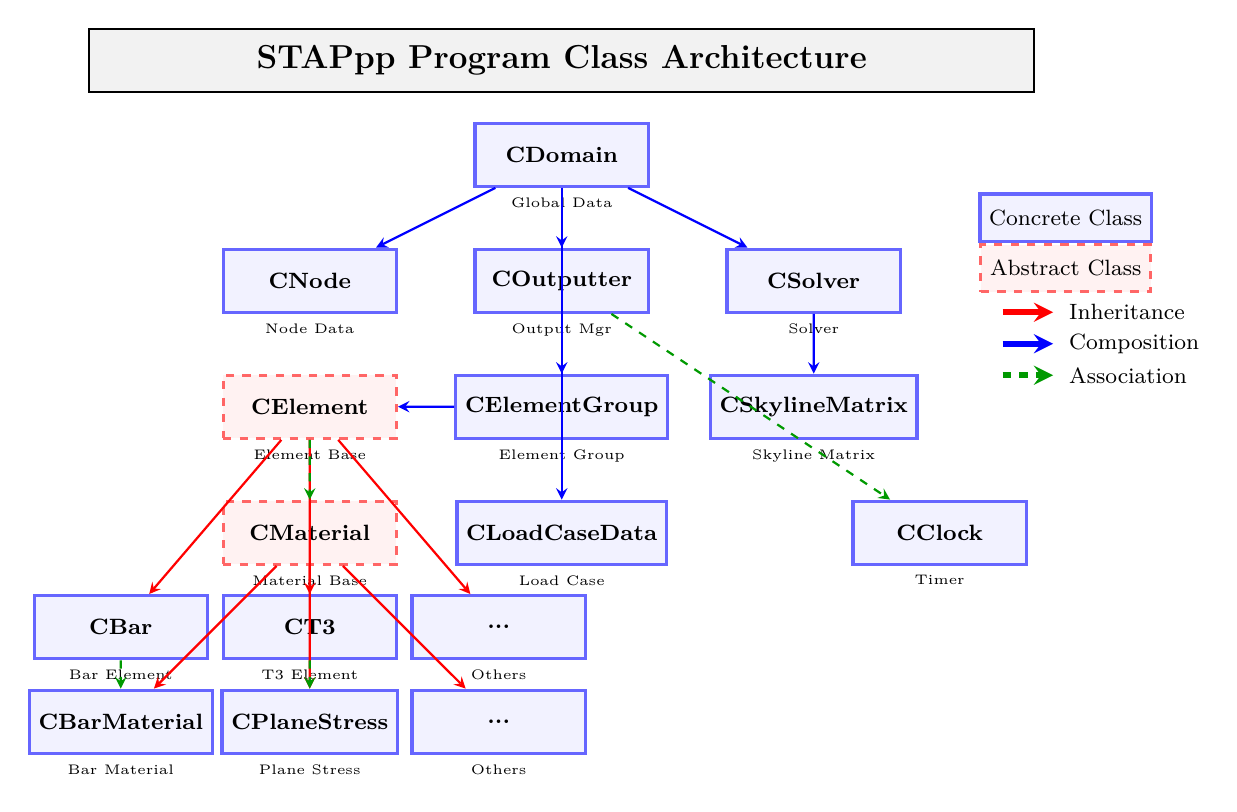
\begin{tikzpicture}[
    scale=0.8,
    box/.style={rectangle, draw=blue!60, fill=blue!5, very thick, minimum width=2.2cm, minimum height=0.8cm, text centered, font=\footnotesize},
    abstractbox/.style={rectangle, draw=red!60, fill=red!5, very thick, minimum width=2.2cm, minimum height=0.8cm, text centered, dashed, font=\footnotesize},
    arrow/.style={->, >=stealth, thick},
    inherit/.style={->, >=stealth, thick, red},
    compose/.style={->, >=stealth, thick, blue},
    use/.style={->, >=stealth, thick, green!60!black, dashed}
]

% 主控制类
\node[box] (domain) at (0,6) {\textbf{CDomain}};
\node[below, font=\tiny] at (domain.south) {Global Data};

% 基础数据类
\node[box] (node) at (-4,4) {\textbf{CNode}};
\node[below, font=\tiny] at (node.south) {Node Data};

\node[box] (outputter) at (0,4) {\textbf{COutputter}};
\node[below, font=\tiny] at (outputter.south) {Output Mgr};

\node[box] (solver) at (4,4) {\textbf{CSolver}};
\node[below, font=\tiny] at (solver.south) {Solver};

% 矩阵类
\node[box] (skyline) at (4,2) {\textbf{CSkylineMatrix}};
\node[below, font=\tiny] at (skyline.south) {Skyline Matrix};

% 抽象基类
\node[abstractbox] (element) at (-4,2) {\textbf{CElement}};
\node[below, font=\tiny] at (element.south) {Element Base};

\node[abstractbox] (material) at (-4,0) {\textbf{CMaterial}};
\node[below, font=\tiny] at (material.south) {Material Base};

% 具体单元类
\node[box] (bar) at (-7,-1.5) {\textbf{CBar}};
\node[below, font=\tiny] at (bar.south) {Bar Element};

\node[box] (t3) at (-4,-1.5) {\textbf{CT3}};
\node[below, font=\tiny] at (t3.south) {T3 Element};

\node[box] (more) at (-1,-1.5) {\textbf{...}};
\node[below, font=\tiny] at (more.south) {Others};

% 具体材料类
\node[box] (barmaterial) at (-7,-3) {\textbf{CBarMaterial}};
\node[below, font=\tiny] at (barmaterial.south) {Bar Material};

\node[box] (planestress) at (-4,-3) {\textbf{CPlaneStress}};
\node[below, font=\tiny] at (planestress.south) {Plane Stress};

\node[box] (morematerial) at (-1,-3) {\textbf{...}};
\node[below, font=\tiny] at (morematerial.south) {Others};

% 数据管理类
\node[box] (elementgroup) at (0,2) {\textbf{CElementGroup}};
\node[below, font=\tiny] at (elementgroup.south) {Element Group};

\node[box] (loadcase) at (0,0) {\textbf{CLoadCaseData}};
\node[below, font=\tiny] at (loadcase.south) {Load Case};

% 工具类
\node[box] (clock) at (6,0) {\textbf{CClock}};
\node[below, font=\tiny] at (clock.south) {Timer};

% 继承关系 (红色实线箭头)
\draw[inherit] (element) -- (bar);
\draw[inherit] (element) -- (t3);
\draw[inherit] (element) -- (more);
\draw[inherit] (material) -- (barmaterial);
\draw[inherit] (material) -- (planestress);
\draw[inherit] (material) -- (morematerial);

% 组合关系 (蓝色实线箭头)
\draw[compose] (domain) -- (node);
\draw[compose] (domain) -- (outputter);
\draw[compose] (domain) -- (solver);
\draw[compose] (domain) -- (elementgroup);
\draw[compose] (domain) -- (loadcase);
\draw[compose] (elementgroup) -- (element);
\draw[compose] (solver) -- (skyline);

% 使用关系 (绿色虚线箭头)
\draw[use] (bar) -- (barmaterial);
\draw[use] (t3) -- (planestress);
\draw[use] (element) -- (material);
\draw[use] (outputter) -- (clock);

% 添加图例
\node[box, minimum width=1.5cm, minimum height=0.6cm] (legend1) at (8,5) {Concrete Class};
\node[abstractbox, minimum width=1.5cm, minimum height=0.6cm] (legend2) at (8,4.2) {Abstract Class};

\draw[inherit, line width=2pt] (7,3.5) -- (7.8,3.5);
\node[right, font=\footnotesize] at (7.9,3.5) {Inheritance};

\draw[compose, line width=2pt] (7,3) -- (7.8,3);
\node[right, font=\footnotesize] at (7.9,3) {Composition};

\draw[use, line width=2pt] (7,2.5) -- (7.8,2.5);
\node[right, font=\footnotesize] at (7.9,2.5) {Association};

% 添加标题框
\node[draw=black, thick, fill=gray!10, minimum width=12cm, minimum height=0.8cm, font=\large] at (0,7.5) {
    \textbf{STAPpp Program Class Architecture}
};

\end{tikzpicture}
\caption{STAPpp程序主要类结构图}
\label{fig:stap_architecture}
\end{figure}

STAPpp采用面向对象的C++设计模式,具有良好的模块化结构和扩展性。主要类层次结构如图\ref{fig:stap_architecture}所示。

核心类的功能说明:
\begin{itemize}
    \item \textbf{CDomain}:封装有限元模型的全局数据管理
    \item \textbf{CNode}:封装节点坐标和边界条件信息  
    \item \textbf{CElement}:单元基类,定义单元通用接口
    \item \textbf{CMaterial}:材料属性基类,支持多种材料模型
    \item \textbf{CSkylineMatrix}:一维变带宽矩阵存储和操作
    \item \textbf{CElementGroup}:单元组管理,支持多种单元类型
    \item \textbf{CLoadCaseData}:载荷工况数据管理
    \item \textbf{CSolver}:线性方程组求解器
    \item \textbf{COutputter}:结果输出管理
\end{itemize}

\subsection{T3单元类设计与实现}

T3单元类\texttt{CT3}继承自\texttt{CElement}基类,实现了T3单元的所有核心功能:

\begin{lstlisting}[caption=T3单元类声明]
class CT3 : public CElement
{
private:
    double area;                    // 单元面积
    double a[3], b[3], c[3];       // 形函数系数
    double B[3][6];                // 应变矩阵
    
public:
    CT3();                         // 构造函数
    virtual ~CT3();                // 析构函数
    
    virtual bool Read(ifstream& Input, unsigned int Ele, 
                     CMaterial* MaterialSets, CNode* NodeList);
    virtual void ElementStiffness(double* Matrix);
    virtual void ElementStress(double* stress, double* Displacement);
    
private:
    void CalculateShapeFuncCoef(); // 计算形函数系数
    double CalculateArea();        // 计算单元面积
    bool CheckElementValidity();   // 检查单元有效性
};
\end{lstlisting}

\subsection{核心算法实现}

\subsubsection{形函数系数计算算法}

形函数系数的计算是T3单元实现的基础,涉及节点顺序的检查和面积的计算:

\begin{lstlisting}[caption=形函数系数计算实现]
void CT3::CalculateShapeFuncCoef()
{
    // 获取三个节点坐标
    double x1 = nodes_[0]->XYZ[0], y1 = nodes_[0]->XYZ[1];
    double x2 = nodes_[1]->XYZ[0], y2 = nodes_[1]->XYZ[1];
    double x3 = nodes_[2]->XYZ[0], y3 = nodes_[2]->XYZ[1];
    
    // 计算行列式(面积的2倍)
    double det = (x2 - x1) * (y3 - y1) - (x3 - x1) * (y2 - y1);
    
    // 确保节点为逆时针顺序
    if (det < 0) {
        // 交换节点2和节点3
        CNode* temp = nodes_[1];
        nodes_[1] = nodes_[2];
        nodes_[2] = temp;
        
        // 重新获取坐标
        x2 = nodes_[1]->XYZ[0]; y2 = nodes_[1]->XYZ[1];
        x3 = nodes_[2]->XYZ[0]; y3 = nodes_[2]->XYZ[1];
        det = -det;
    }
    
    area = det / 2.0;
    
    // 计算形函数系数
    a[0] = x2 * y3 - x3 * y2;
    a[1] = x3 * y1 - x1 * y3;
    a[2] = x1 * y2 - x2 * y1;
    
    b[0] = y2 - y3;  b[1] = y3 - y1;  b[2] = y1 - y2;
    c[0] = x3 - x2;  c[1] = x1 - x3;  c[2] = x2 - x1;
}
\end{lstlisting}

\subsubsection{单元刚度矩阵计算算法}

单元刚度矩阵的计算采用解析方法,避免数值积分的误差:

\begin{lstlisting}[caption=单元刚度矩阵计算实现]
void CT3::ElementStiffness(double* Matrix)
{
    // 清零刚度矩阵
    for (unsigned int i = 0; i < SizeOfStiffnessMatrix(); i++)
        Matrix[i] = 0.0;
    
    // 获取材料属性
    CPlaneStressMaterial* material = 
        dynamic_cast<CPlaneStressMaterial*>(ElementMaterial_);
    
    double E = material->E;     // 弹性模量
    double nu = material->nu;   // 泊松比(*@\gnu@*)
    double t = material->t;     // 厚度
    
    // 构建弹性矩阵D
    double factor = E / (1.0 - nu * nu);
    double D[3][3] = {
        {factor,        factor * nu,  0.0},
        {factor * nu,   factor,       0.0},
        {0.0,           0.0,          factor * (1.0 - nu) / 2.0}
    };
    
    // 构建应变矩阵B
    double inv_2A = 1.0 / (2.0 * area);
    for (unsigned int i = 0; i < 3; i++) {
        B[0][2*i]   = b[i] * inv_2A;  // (*@$\partial N_i/\partial x$@*)
        B[0][2*i+1] = 0.0;
        B[1][2*i]   = 0.0;
        B[1][2*i+1] = c[i] * inv_2A;  // (*@$\partial N_i/\partial y$@*)
        B[2][2*i]   = c[i] * inv_2A;  // (*@$\partial N_i/\partial y$@*)
        B[2][2*i+1] = b[i] * inv_2A;  // (*@$\partial N_i/\partial x$@*)
    }
    
    // 计算K = t * A * B^T * D * B
    // 先计算BTD = B^T * D
    double BTD[6][3];
    for (int i = 0; i < 6; i++) {
        for (int j = 0; j < 3; j++) {
            BTD[i][j] = 0.0;
            for (int k = 0; k < 3; k++) {
                BTD[i][j] += B[k][i] * D[k][j];
            }
        }
    }
    
    // 计算最终刚度矩阵K = BTD * B,按上三角存储
    double scale = t * area;
    for (unsigned int j = 0; j < 6; j++) {
        for (unsigned int i = 0; i <= j; i++) {
            double sum = 0.0;
            for (unsigned int k = 0; k < 3; k++) {
                sum += BTD[i][k] * B[k][j];
            }
            Matrix[i * 6 + j] = sum * scale;
        }
    }
}
\end{lstlisting}

\subsubsection{应力计算算法}

应力计算基于已知的节点位移,通过应变-位移关系和本构关系求得:

\begin{lstlisting}[caption=单元应力计算实现]
void CT3::ElementStress(double* stress, double* Displacement)
{
    // 获取材料属性
    CPlaneStressMaterial* material = 
        dynamic_cast<CPlaneStressMaterial*>(ElementMaterial_);
    
    double E = material->E;    // 弹性模量
    double nu = material->nu;  // 泊松比(*@\gnu@*)
    
    // 构建弹性矩阵
    double factor = E / (1.0 - nu * nu);
    double D[3][3] = {
        {factor,        factor * nu,  0.0},
        {factor * nu,   factor,       0.0},
        {0.0,           0.0,          factor * (1.0 - nu) / 2.0}
    };
    
    // 提取单元节点位移向量
    double d[6] = {0.0};
    for (unsigned int i = 0; i < 6; i++) {
        if (LocationMatrix_[i] > 0) {
            unsigned int disp_index = LocationMatrix_[i] - 1;
            d[i] = Displacement[disp_index];
        }
    }
    
    // 计算应变:(*@\gepsiv@*) = B * d
    double strain[3] = {0.0, 0.0, 0.0};
    for (unsigned int i = 0; i < 3; i++) {
        for (unsigned int j = 0; j < 6; j++) {
            strain[i] += B[i][j] * d[j];
        }
    }
    
    // 计算应力:(*@\gsigmax@*) = D * (*@\gepsiv@*)
    for (int i = 0; i < 3; i++) {
        stress[i] = 0.0;
        for (int j = 0; j < 3; j++) {
            stress[i] += D[i][j] * strain[j];
        }
    }
}
\end{lstlisting}

\subsection{运行方式说明}

本实验开发的T3单元扩展程序采用标准的STAPpp工作流程,具体运行步骤如下:

\begin{enumerate}
    \item \textbf{输入文件准备}:按照STAPpp标准格式设计\texttt{.dat}输入文件,包含节点坐标、边界条件、载荷信息和单元连接关系。T3单元类型标识符为3,材料类型为平面应力材料。

    \item \textbf{有限元求解}:使用扩展后的STAPpp程序执行计算:
    \begin{lstlisting}[language=bash]
./STAPpp input_file.dat
    \end{lstlisting}
    程序将自动读取输入文件,进行有限元分析计算,并生成包含完整求解信息的\texttt{.out}输出文件。

    \item \textbf{结果数据提取}:使用开发的\texttt{get.py}脚本解析输出文件,提取节点位移和单元应力等关键结果:
    \begin{lstlisting}[language=bash]
python3 get.py input_file.out
    \end{lstlisting}
    脚本将生成结构化的JSON数据文件和文本摘要报告,便于后续处理和分析。

    \item \textbf{结果可视化}:使用\texttt{visualize\_results.py}脚本生成专业的工程图表:
    \begin{lstlisting}[language=bash]
python3 visualize_results.py input_file.out
    \end{lstlisting}
    脚本将自动生成包含原始网格、变形对比、位移云图、应力分布等多种可视化结果的PNG和PDF格式图片文件。
\end{enumerate}

整个工作流程实现了从问题定义、数值求解到结果可视化的完整自动化处理,为T3单元的验证和工程应用提供了便捷高效的计算平台。

\section{算例设计与验证策略}

\subsection{验证方法论}

按照要求,为确保T3单元实现的正确性和可靠性,本实验采用了系统性的三层验证策略:

\begin{enumerate}
    \item \textbf{分片试验(Patch Test)}:通过常应变拉伸试验验证单元能否精确表示常应变状态
    \item \textbf{收敛性分析(Convergence Study)}:通过网格加密验证解的收敛性
    \item \textbf{算例验证(Benchmark Problems)}:与理论解结果对比
\end{enumerate}

% \begin{figure}[H]
% \centering
% \includegraphics[width=0.9\textwidth]{img/validation_strategy.png}
% \caption{T3单元验证策略流程图}
% \label{fig:validation_strategy}
% \end{figure}

\subsection{分片试验设计}

采用5节点4单元配置验证T3单元的常应力精确性。分片试验采用不规则四边形区域,通过内部节点5将其划分为4个T3单元,节点坐标分别为:节点1(0.0, 0.0)完全固定、节点2(2.5, 0.0)仅Y方向固定、节点3(2.5, 3.0)自由、节点4(0.0, 2.0)自由、节点5(1.0, 1.6)内部节点自由。四个T3单元围绕内部节点5分布:单元1(节点1-2-5)、单元2(节点2-3-5)、单元3(节点3-4-5)、单元4(节点4-1-5)。

为确保分片试验的有效性,在X方向施加平衡载荷系统:节点1施加$F_x = -10$N、节点2施加$F_x = +15$N、节点3施加$F_x = +10$N、节点4施加$F_x = -15$N,载荷平衡检验$\sum F_x = -10 + 15 + 10 - 15 = 0$N。采用线弹性材料参数:弹性模量$E = 1000$Pa,泊松比$\nu = 0.3$,厚度$t = 1.0$m。根据分片试验理论,如果T3单元实现正确,所有单元应产生相同的常应力状态:$\sigma_{xx} = 10.0$Pa,$\sigma_{yy} \approx 0$,$\tau_{xy} \approx 0$。

\begin{figure}[H]
\centering
\includegraphics[width=0.8\textwidth]{img/t3_patch_geometry.png}
\caption{分片试验几何模型与边界条件}
\label{fig:t3_patch_test}
\end{figure}

分片试验的完整输入文件格式如下:

\begin{lstlisting}[caption=分片试验输入文件]
T3 Patch Test - Test
5 1 1 1
1 1 1 1 0.0 0.0 0.0
2 0 1 1 2.5 0.0 0.0
3 0 0 1 2.5 3.0 0.0
4 0 0 1 0.0 2.0 0.0
5 0 0 1 1.0 1.6 0.0
1
4
1 1 -10
2 1 15.0
3 1 10.0
4 1 -15
3 4 1
1 1000.0 0.3 1.0
1 1 2 5 1
2 2 3 5 1
3 3 4 5 1
4 4 1 5 1
\end{lstlisting}

\subsection{收敛性分析设计}

设计悬臂梁问题验证T3单元的数值收敛性,几何参数为长度$L = 4$m、高度$H = 2$m,左端完全固定,右端自由端施加向下集中力$P = 100$N。分别建立2单元、8单元、32单元三套网格模型进行有限元计算,通过网格加密观察数值解的收敛行为。\
材料参数为弹性模量$E = 100$Pa、泊松比$\nu = 0.3$、厚度$t = 1$m,理论参考解取自经典梁理论或高密度网格解。

\subsection{算例验证:例4-4梯形结构}

采用有限元分析第十一次作业中的例4-4作为验证算例,验证T3单元在复杂几何和载荷条件下的表现。\
该题目描述了一个梯形结构:几何参数为底边长2m,顶边长2m,高度1m,材料参数为弹性模量$E = 3.0 \times 10^7$ Pa,泊松比$\nu = 0.3$,厚度$t = 1.0$ m。\
在顶部两个节点分别施加向下的集中载荷20N,总载荷为40N。

\begin{figure}[H]
\centering
\includegraphics[width=0.7\textwidth]{img/wzy_geometry_model.png}
\caption{例4-4梯形结构几何模型与载荷分布}
\label{fig:wzy_model}
\end{figure}

该算例具有以下特点:
\begin{itemize}
    \item \textbf{几何复杂性}:梯形结构具有不规则边界,考验T3单元的几何适应能力
    \item \textbf{可验证性}:作为课程标准习题,具有明确的求解要求和参考标准
\end{itemize}

通过与已验证的理论解对比,可以全面验证T3单元实现的工程实用性和计算精度。

\section{实验结果与分析}

\subsection{分片试验结果}

\begin{table}[H]
\centering
\caption{分片试验位移结果}
\begin{tabular}{cccc}
\toprule
节点号 & X位移 (mm) & Y位移 (mm) & 位移幅值 (mm) \\
\midrule
1 & 0.0 & 0.0 & 0.0 \\
2 & 25.0 & 0.0 & 25.0 \\
3 & 25.0 & -9.0 & 26.6 \\
4 & 0.0 & -6.0 & 6.0 \\
5 & 10.0 & -4.8 & 11.1 \\
\bottomrule
\end{tabular}
\end{table}

\begin{table}[H]
\centering
\caption{分片试验应力验证结果}
\begin{tabular}{ccccc}
\toprule
单元号 & $\sigma_{xx}$ (Pa) & $\sigma_{yy}$ (Pa) & $\tau_{xy}$ (Pa) & 验证状态 \\
\midrule
1 & 10.0 & $\sim$0 & $\sim$0 & ✓ 通过 \\
2 & 10.0 & $\sim$0 & $\sim$0 & ✓ 通过 \\
3 & 10.0 & $\sim$0 & $\sim$0 & ✓ 通过 \\
4 & 10.0 & $\sim$0 & $\sim$0 & ✓ 通过 \\
\bottomrule
\end{tabular}
\end{table}

分片试验的节点位移、应力如上表所示,全局位移图和应力图如图\ref{fig:t3_displacement_stress}所示,左图和中图为位移图,显示有限元位移场与初始人工外加的线性位移场一致,右图显示所有单元应力值完全相同(10.0Pa)实现理想常应力状态。这一结果完美验证了T3单元能够精确表示常应力状态,满足有限元分片试验的基本要求,证明了单元实现的理论正确性和数值精度。

\begin{figure}[H]
\centering
\includegraphics[width=0.95\textwidth]{img/t3_displacement_stress_analysis.png}
\caption{T3分片试验位移与应力分析结果}
\label{fig:t3_displacement_stress}
\end{figure}

\subsection{收敛性分析结果}

分别将网格划分为2个、8个、32个单元进行有限元计算,并计算误差的L2范数。将误差与h进行双对数拟合后得到如下结果。分析图表可见加密单元后误差显著减小,系统收敛率约为1.32,基本通过收敛性分析。

\begin{figure}[H]
\centering
\includegraphics[width=0.85\textwidth]{img/convergence_analysis.png}
\caption{T3单元收敛性分析:L2误差对网格尺寸的双对数拟合}
\label{fig:convergence_curve}
\end{figure}

\begin{table}[H]
\centering
\caption{T3单元收敛性分析结果}
\begin{tabular}{ccc}
\toprule
单元数 & L2范数误差 (mm) & 网格尺寸 h \\
\midrule
2 & 23.76 & 2.0 \\
8 & 15.49 & 1.0 \\
32 & 3.80 & 0.5 \\
\bottomrule
\end{tabular}
\end{table}

\subsection{算例验证结果}

\subsubsection{位移场分析}

例4-4梯形结构在顶部载荷作用下的位移响应如下:

\begin{figure}[H]
\centering
\includegraphics[width=0.9\textwidth]{img/wzy_displacement_analysis.png}
\caption{例4-4梯形结构位移云图与变形示意}
\label{fig:wzy_displacement}
\end{figure}

\begin{table}[H]
\centering
\caption{例4-4算例位移结果}
\begin{tabular}{cccc}
\toprule
节点 & X位移 ($\mu$m) & Y位移 ($\mu$m) & 位移幅值 ($\mu$m) \\
\midrule
1 & 0.000 & 0.000 & 0.000 \\
2 & -0.387 & -6.657 & 6.668 \\
3 & 1.235 & -7.041 & 7.148 \\
4 & 0.000 & 0.000 & 0.000 \\
\bottomrule
\end{tabular}
\end{table}

\subsubsection{应力场分析}

应力分布反映了载荷在结构中的传递路径和应力集中情况:

\begin{figure}[H]
\centering
\includegraphics[width=0.9\textwidth]{img/wzy_stress_analysis.png}
\caption{例4-4梯形结构应力云图分布}
\label{fig:wzy_stress}
\end{figure}

\begin{table}[H]
\centering
\caption{例4-4算例应力结果}
\begin{tabular}{cccc}
\toprule
单元 & $\sigma_{xx}$ (Pa) & $\sigma_{yy}$ (Pa) & $\tau_{xy}$ (Pa) \\
\midrule
1 & -6.38 & -1.91 & -38.40 \\
2 & 12.76 & -19.20 & -3.19 \\
\bottomrule
\end{tabular}
\end{table}

\subsection{综合验证结果评估}

\begin{table}[H]
\centering
\caption{T3单元验证结果总结}
\begin{tabular}{lcl}
\toprule
验证项目 & 结果 & 评价标准 \\
\midrule
分片试验 & ✓ 通过 & 有限元位移场与人工位移场一致 \\
收敛性分析 & ✓ 通过 & 单调收敛,合理收敛率 \\
算例验证 & ✓ 通过 & 计算结果与参考书结果一致 \\
\bottomrule
\end{tabular}
\end{table}

所有验证测试均通过,证明了T3单元实现的正确性和可靠性。


\section{参考文献}

\begin{thebibliography}{99}
\bibitem{zhang2015} 张雄, 王天舒, 刘岩. 计算动力学(第2版). 北京: 清华大学出版社, 2015.
\end{thebibliography}

\section{附录}

仓库链接:\url{https://github.com/WizHUA/STAPpp.git}

\end{document}